\documentclass[a4paper,11pt, notitlepage]{article}

\usepackage[utf8]{inputenc}
\usepackage[T1]{fontenc}

\usepackage[top=2.5cm, bottom=3cm, left=3cm, right=3cm, headsep=14pt]{geometry}
\usepackage{graphicx}
\graphicspath{{images/}}
\usepackage[export]{adjustbox}

\usepackage{datetime}
\usepackage{float}
\usepackage{a4wide}
\usepackage[super]{nth}
\usepackage{mathtools}
\usepackage{hyperref}
\usepackage{fancyvrb}
\usepackage{booktabs}
\usepackage{multirow}
\usepackage{caption}

\usepackage{natbib}
\bibliographystyle{unsrt}


\setlength{\parskip}{0.5em}

\begin{document}

\title{
\vspace{-3cm}
Report 3 - CUDA}
\author{Nguyen Nhu Khoa - M.ICT.06.003}
\maketitle

\pagestyle{plain}
\setcounter{page}{1}

\vspace{-1cm}
\newdate{date}{31}{10}{2017}
\noindent

\section{Labwork Implementation}

Kernel:
\begin{flushleft}
\small
\begin{BVerbatim}
__global__ void grayscaleConvert(char* input, char* output, int imagePixelCount){
        for (int i = 0; i < imagePixelCount; i++) {
            output[i * 3] = (char) (((int) input[i * 3] + (int) input[i * 3 + 1] +
                                          (int) input[i * 3 + 2]) / 3);
            output[i * 3 + 1] = output[i * 3];
            output[i * 3 + 2] = output[i * 3];
        }
}
\end{BVerbatim}
\end{flushleft}
~\\
Labwork3 function:
\begin{flushleft}
\small
\begin{BVerbatim}
void Labwork::labwork3_GPU() {
    int pixelCount = inputImage->width * inputImage->height;
    outputImage = static_cast<char *>(malloc(pixelCount * 3)); 

    char *blockSizeEnv = getenv("LW3_CUDA_BLOCK_SIZE");
    int blockSize = atoi(blockSizeEnv);
    long numBlock = pixelCount/blockSize;

    char *cuInput, *cuOutput;
    cudaMalloc(&cuInput, pixelCount*3*sizeof(char));
    cudaMalloc(&cuOutput, pixelCount*3*sizeof(char));
    
    cudaMemcpy(cuInput, inputImage->buffer, pixelCount*3*sizeof(char), cudaMemcpyHostToDevice);
    
    for (int j = 0; j < 100; j++) {     // let's do it 100 times, otherwise it's too fast!
    	grayscaleConvert<<<numBlock, blockSize>>>(cuInput, cuOutput, pixelCount);
    }
    cudaMemcpy(outputImage, cuOutput, pixelCount*3*sizeof(char), cudaMemcpyDeviceToHost);
    
    cudaFree(cuOutput);
    cudaFree(cuInput);
}
\end{BVerbatim}
\end{flushleft}

\section{Speedup}
Compare to the original version of the function, which was run on CPU without any paralellism, the new function using CUDA with block size of 64 has a speedup of roughly 43x. \\

\section{Other block size config}
\begin{figure}[H]
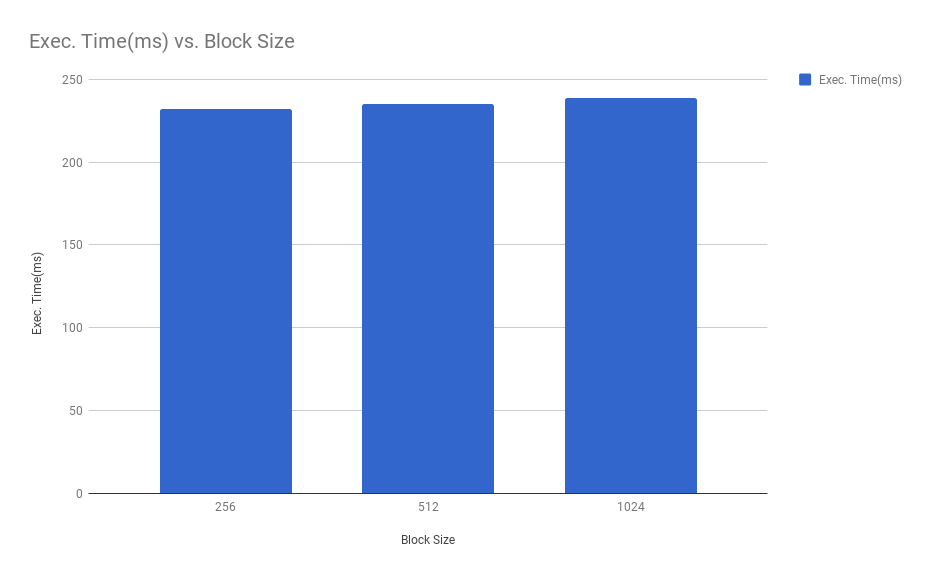
\includegraphics[width=15cm]{chart-cuda-block-size.png}
\centering
\caption{Block Size Performance Comparison}
\end{figure}
~\\
Here, there aren't too much differences in terms of performance when the number of block size changes. This might be due to the program is simple that other config of block size doesn't matter too much. \\
\end{document}